\documentclass{article}
\usepackage{amsmath}
\usepackage{graphicx}
\usepackage{float}
\usepackage{hyperref}
\usepackage{caption}

\title{CS 5720: Design and Analysis of Algorithms \\ Project 0 Report}
\author{Rachel Koch}
\date{\today}

\begin{document}

\maketitle

\section{Introduction}

The goal of this project is to visualize and empirically test the order of growth of different functions using Python. We will plot several functions and their ratios to determine if they have the same or different orders of growth. This report contains plots and interpretations for each deliverable specified in the project assignment.

\section{Attributions}

ChatGPT file changes: \textit{second\_code.py}

\begin{quote}
Changed the name of the file\\
Added comments to functions identifying deliverables\\
Defined the interval size for the ranges of n\\
Added labels to the plots for deliverable 1\\
Renamed output plots and files\\
Changed deliverable 4 to start at 1 instead of 2\\
Changed the first graphs of deliverable 5 to start at 1
\end{quote}
ChatGPT file changes: \textit{main.tex}

\begin{quote}
Changed the name of the file\\
Swapped out the images for images generated by my program\\
Wrote my own observations of the graphs if they differed from ChatGPTs
\end{quote}

\section{Deliverable 1: Visualizing Functions with the Same Order of Growth}

\subsection{Functions}
The functions under consideration are:
\[
f(n) = \frac{1}{2}n(n - 1) + 10, \quad g(n) = n^2
\]

\subsection{Plots and Interpretation}

\begin{figure}[H]
    \centering
    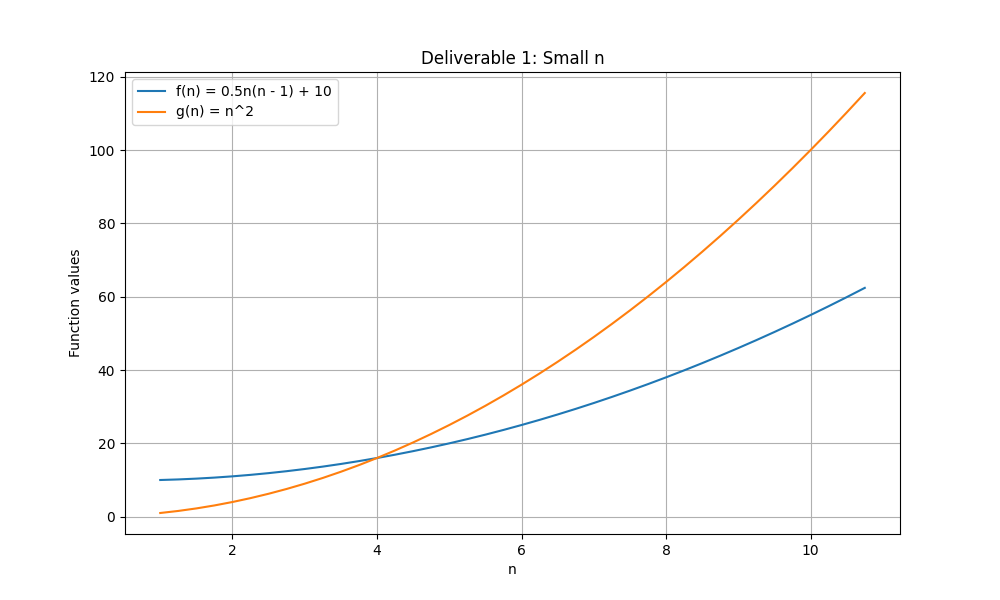
\includegraphics[width=\textwidth]{plot_deliverable1_smalln.png}
    \caption{Plot of $f(n)$ and $g(n)$ for $n$ ranging from 1 to 10.}
    \label{fig:fn_gn_1_10}
\end{figure}

\begin{figure}[H]
    \centering
    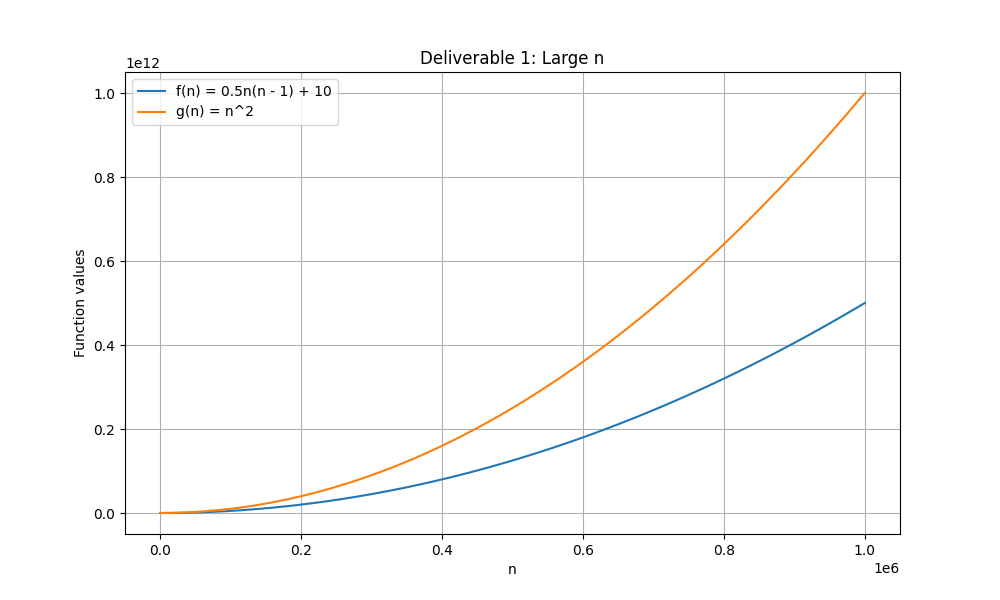
\includegraphics[width=\textwidth]{plot_deliverable1_largen.png}
    \caption{Plot of $f(n)$ and $g(n)$ for $n$ ranging from 1 to $10^6$.}
    \label{fig:fn_gn_1_10e6}
\end{figure}

\textbf{Interpretation:} In Figure \ref{fig:fn_gn_1_10}, the functions $f(n)$ and $g(n)$ appear to have a different growth rate for small values of $n$. It seems like $f(n)$ grows faster than $g(n)$. However, Figure \ref{fig:fn_gn_1_10e6}, as $n$ becomes large, shows that neither function approaches zero or grows faster than the other. This indicates that they are in the same order of growth, $\Theta(n^2)$.

\section{Deliverable 2: Empirical Limit Test}

\subsection{Empirical Limit Test}

We plot the ratio $\frac{f(n)}{g(n)}$ to empirically test the limit:

\begin{figure}[H]
    \centering
    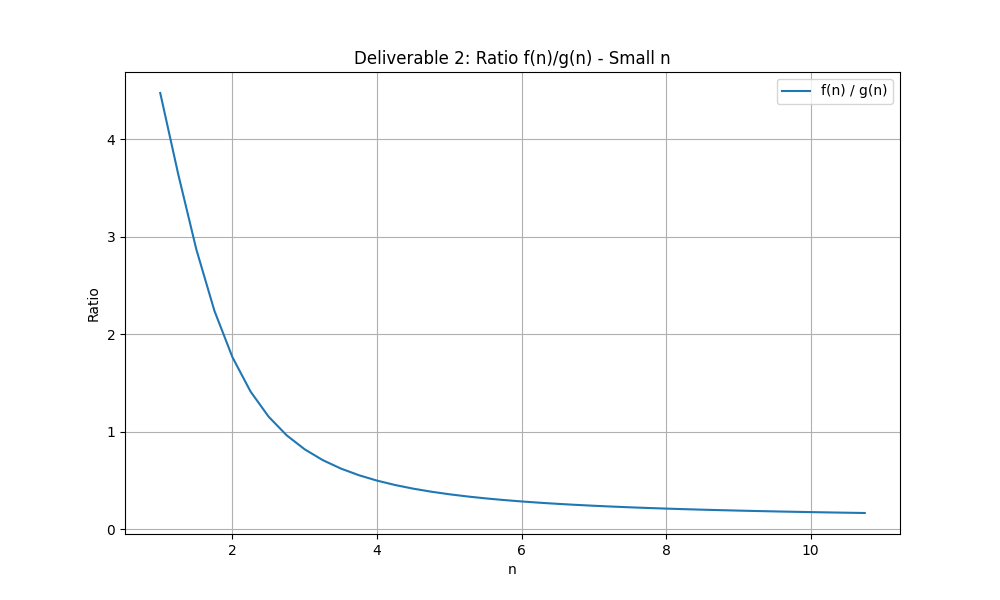
\includegraphics[width=\textwidth]{plot_deliverable2_ratio_smalln.png}
    \caption{Plot of $\frac{f(n)}{g(n)}$ for $n$ ranging from 1 to 10.}
    \label{fig:ratio_fn_gn_1_10}
\end{figure}

\begin{figure}[H]
    \centering
    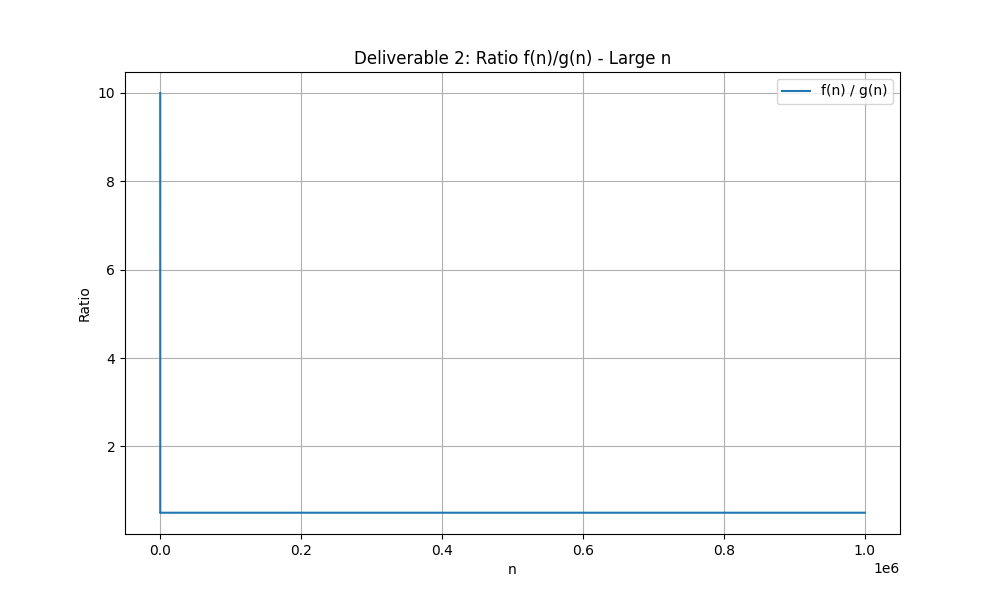
\includegraphics[width=\textwidth]{plot_deliverable2_ratio_largen.png}
    \caption{Plot of $\frac{f(n)}{g(n)}$ for $n$ ranging from 1 to $10^6$.}
    \label{fig:ratio_fn_gn_1_10e6}
\end{figure}

\textbf{Interpretation:} In Figure \ref{fig:ratio_fn_gn_1_10}, the ratio $\frac{f(n)}{g(n)}$ varies significantly for small values of $n$. In Figure \ref{fig:ratio_fn_gn_1_10e6}, the ratio approaches a constant value as $n$ increases, confirming that $f(n)$ and $g(n)$ are indeed in the same order of growth.

\section{Deliverable 3: Functions with Different Orders of Growth}

\subsection{Functions}
\[
f(n) = \sqrt{n^5 + 3n + 1}, \quad g(n) = 5n^2
\]

\subsection{Plots and Interpretation}

\begin{figure}[H]
    \centering
    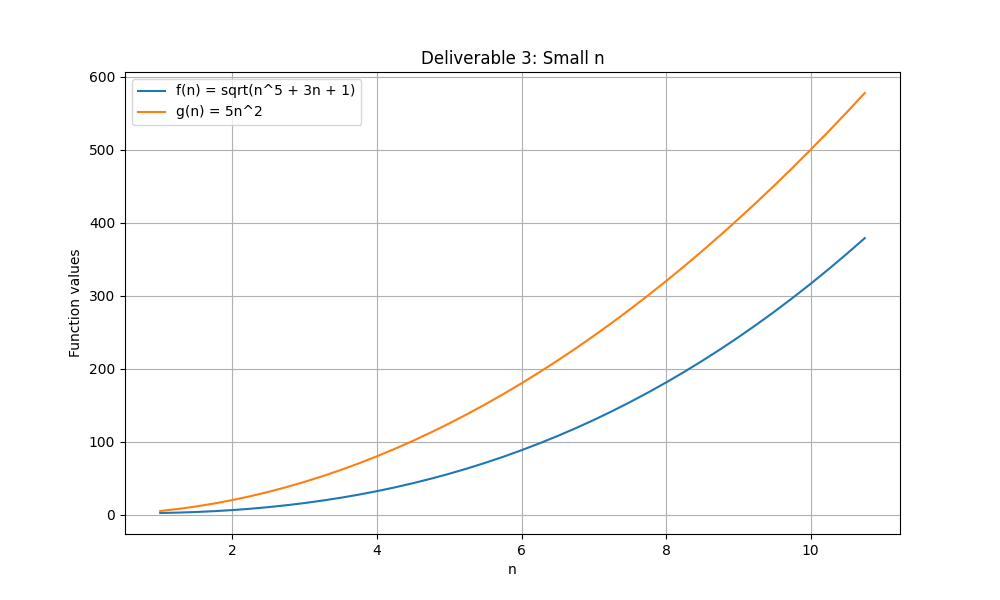
\includegraphics[width=\textwidth]{plot_deliverable3_smalln.png}
    \caption{Plot of $f(n)$ and $g(n)$ for $n$ ranging from 1 to 10.}
    \label{fig:fn2_gn2_1_10}
\end{figure}

\begin{figure}[H]
    \centering
    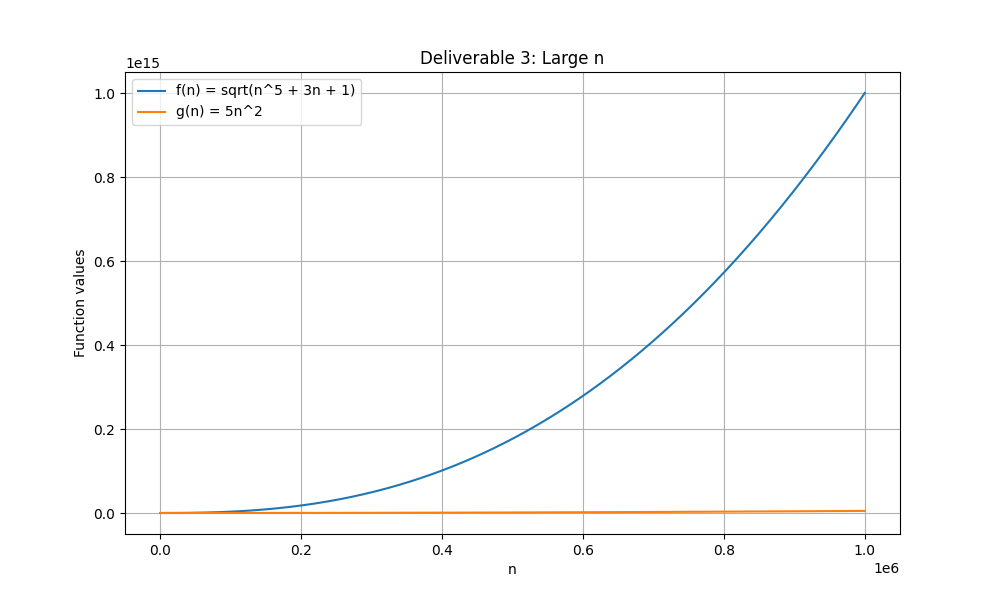
\includegraphics[width=\textwidth]{plot_deliverable3_largen.png}
    \caption{Plot of $f(n)$ and $g(n)$ for $n$ ranging from 1 to $10^6$.}
    \label{fig:fn2_gn2_1_10e6}
\end{figure}

\begin{figure}[H]
    \centering
    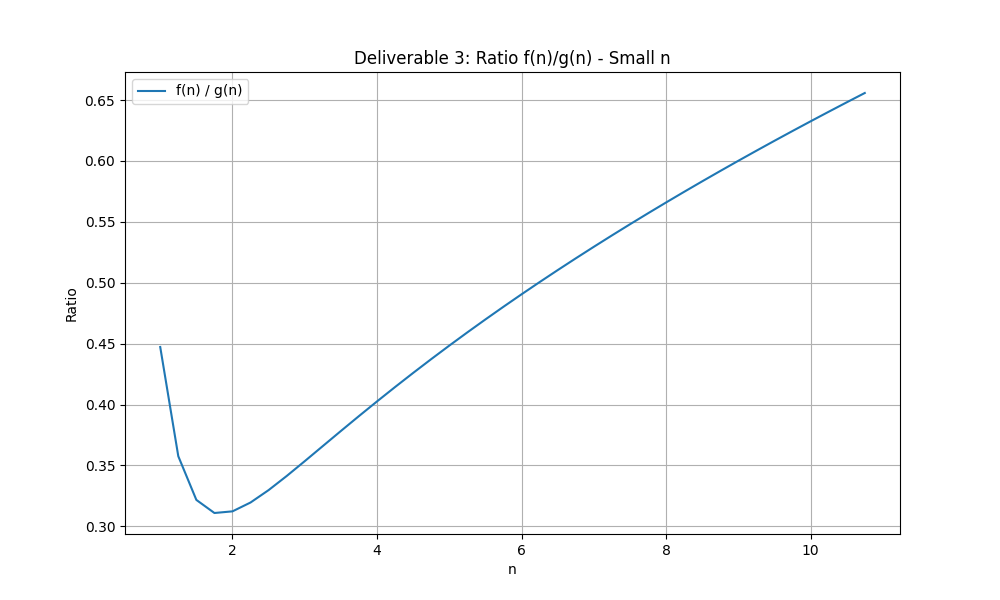
\includegraphics[width=\textwidth]{plot_deliverable3_ratio_smalln.png}
    \caption{Plot of $\frac{f(n)}{g(n)}$ for $n$ ranging from 1 to 10.}
    \label{fig:ratio_fn2_gn2_1_10}
\end{figure}

\begin{figure}[H]
    \centering
    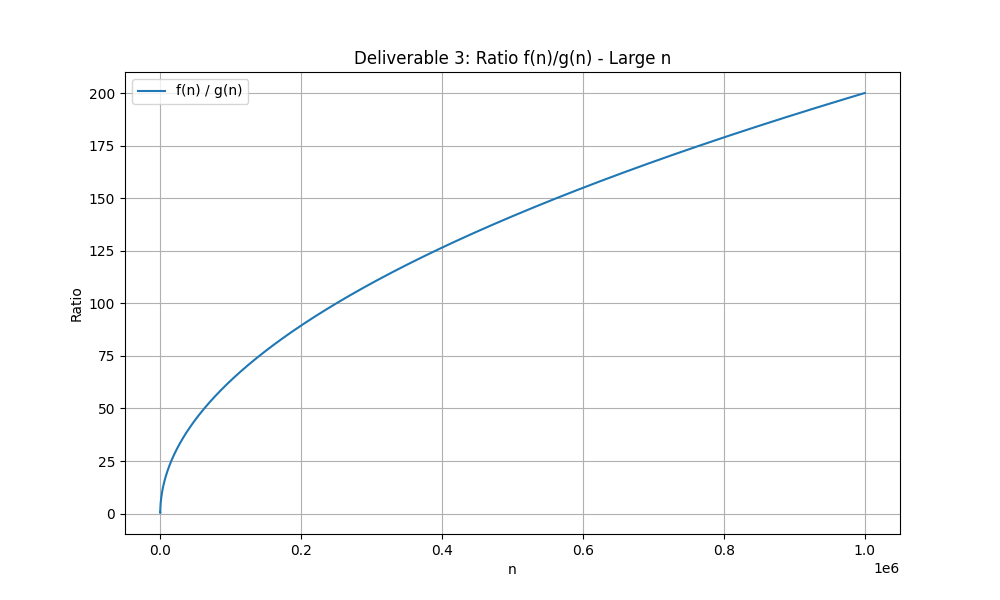
\includegraphics[width=\textwidth]{plot_deliverable3_ratio_largen.png}
    \caption{Plot of $\frac{f(n)}{g(n)}$ for $n$ ranging from 1 to $10^6$.}
    \label{fig:ratio_fn2_gn2_1_10e6}
\end{figure}

\textbf{Interpretation:} The plots containing large values of $n$ clearly show that $f(n)$ grows faster than $g(n)$. Initially, it looked like $g(n)$ might grow faster, as shown with small values of $n$. However, the ratio charts confirmed that $f(n)$ and $g(n)$ have different orders of growth, as their ratio never approaches a constant value. In fact, given that the ratio is continually increasing, we can say that $f(n)$ definitively outperforms $g(n)$. Mathematically, this can be confirmed by calculating their orders of growth: $f(n) \in \Theta(n^{2.5})$ while $g(n) \in \Theta(n^2)$. 

\section{Deliverable 4: Functions with Slower Growth Rates}

\subsection{Functions}
\[
f(n) = \log n, \quad g(n) = \sqrt{n}
\]

\subsection{Plots and Interpretation}

\begin{figure}[H]
    \centering
    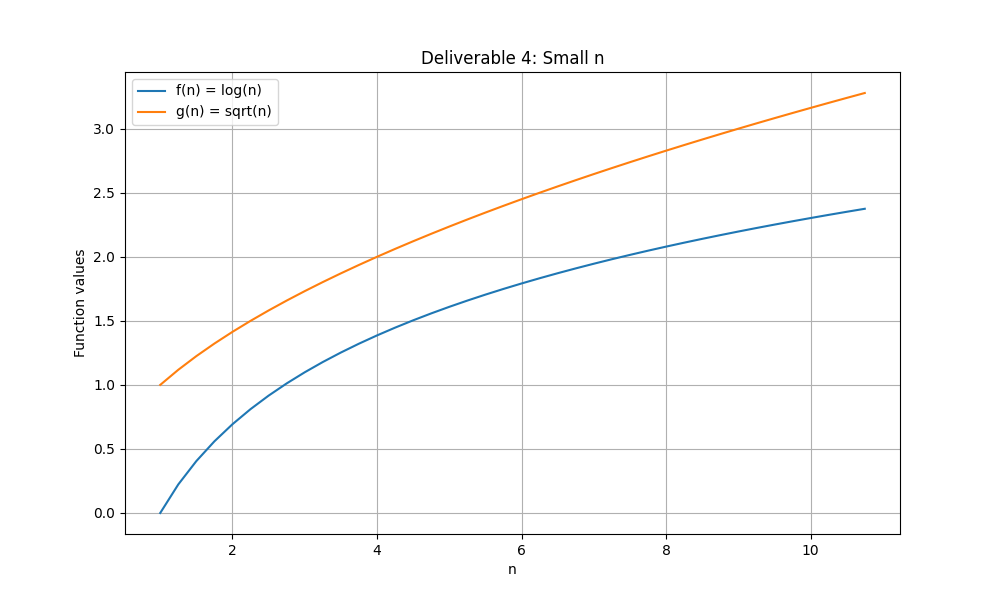
\includegraphics[width=\textwidth]{plot_deliverable4_smalln.png}
    \caption{Plot of $f(n)$ and $g(n)$ for $n$ ranging from 1 to 10.}
    \label{fig:fn3_gn3_2_10}
\end{figure}

\begin{figure}[H]
    \centering
    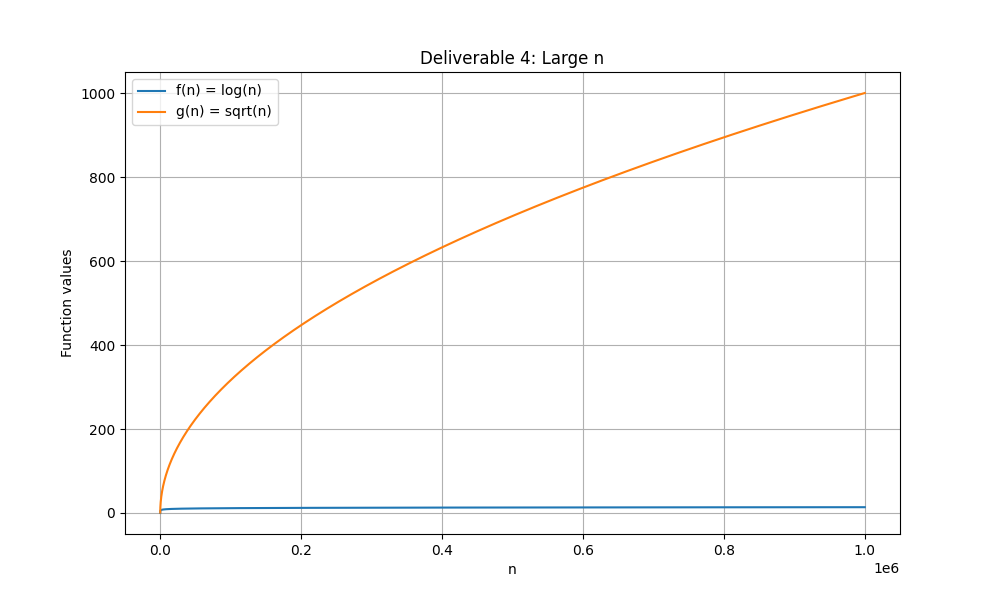
\includegraphics[width=\textwidth]{plot_deliverable4_largen.png}
    \caption{Plot of $f(n)$ and $g(n)$ for $n$ ranging from 1 to $10^6$.}
    \label{fig:fn3_gn3_2_10e6}
\end{figure}

\begin{figure}[H]
    \centering
    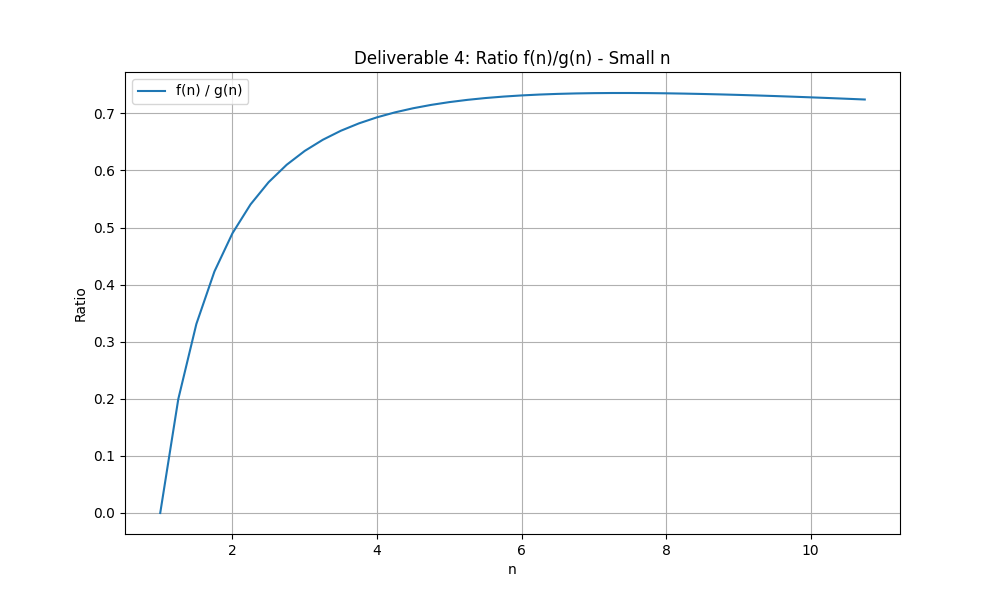
\includegraphics[width=\textwidth]{plot_deliverable4_ratio_smalln.png}
    \caption{Plot of $\frac{f(n)}{g(n)}$ for $n$ ranging from 1 to 10.}
    \label{fig:ratio_fn3_gn3_2_10}
\end{figure}

\begin{figure}[H]
    \centering
    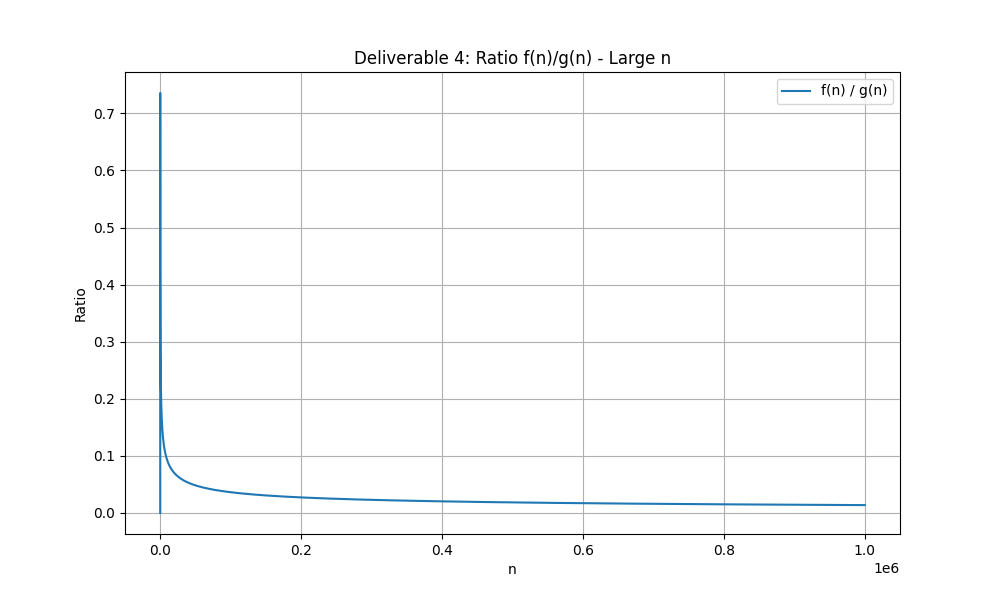
\includegraphics[width=\textwidth]{plot_deliverable4_ratio_largen.png}
    \caption{Plot of $\frac{f(n)}{g(n)}$ for $n$ ranging from 1 to $10^6$.}
    \label{fig:ratio_fn3_gn3_2_10e6}
\end{figure}

\textbf{Interpretation:} Even for small values of $n$, it appears that $g(n)$ grows faster. Only slightly at first, but over larger values of $n$ it's clear that $f(n)$ grows much slower than $g(n)$. The ratio plots are a little more difficult to understand, because the initial analysis of smaller values of n indicates that $f(n)$ outperforms $g(n)$. However, it can be seen that $g(n)$ quickly makes up the difference and slowly outpaces $f(n)$ in the long term. Therefore, $g(n)$ has a greater order of growth than $f(n)$. Again, this can be confirmed mathematically by calculating their orders of growth: $g(n) \in \Theta(\sqrt{n})$ and $f(n) \in \Theta(\log n)$.

\section{Deliverable 5: Logarithmic Functions with the Same Order of Growth}

\subsection{Functions}
\[
f(n) = \log_2 n, \quad g(n) = \log_{10} n
\]

\subsection{Plots and Interpretation}

\begin{figure}[H]
    \centering
    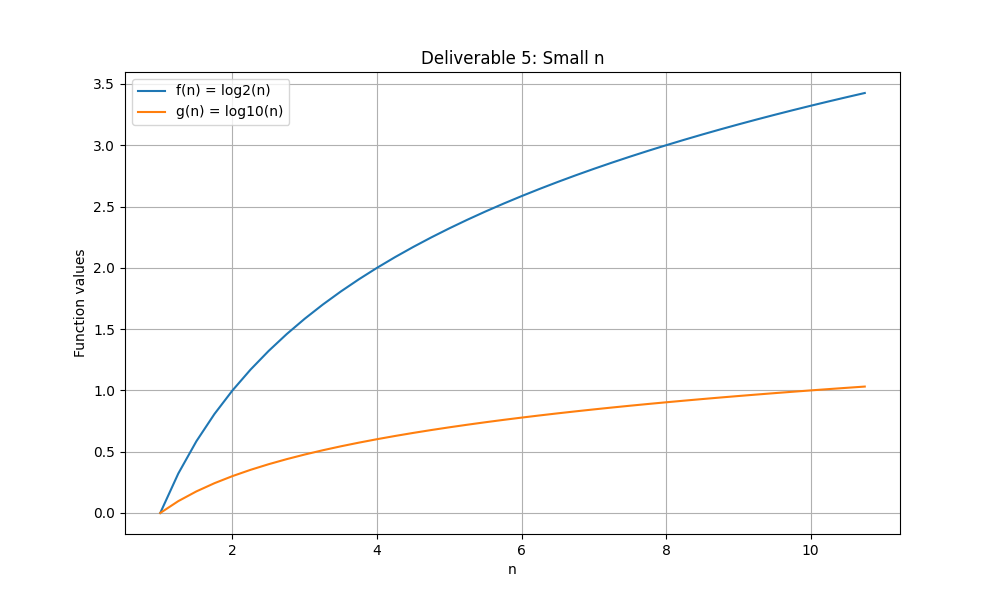
\includegraphics[width=\textwidth]{plot_deliverable5_smalln.png}
    \caption{Plot of $f(n)$ and $g(n)$ for $n$ ranging from 2 to 10.}
    \label{fig:fn4_gn4_2_10}
\end{figure}

\begin{figure}[H]
    \centering
    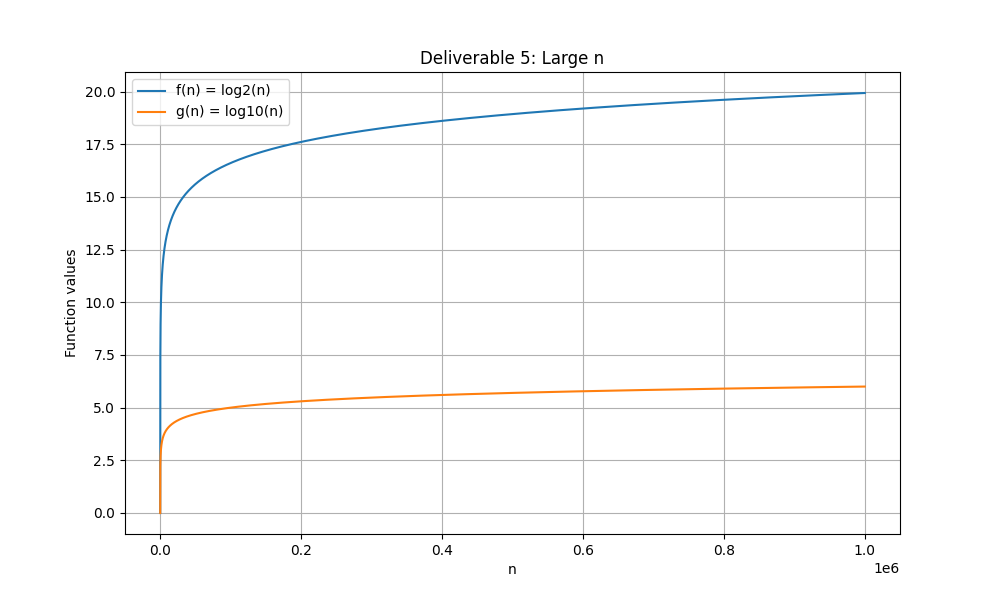
\includegraphics[width=\textwidth]{plot_deliverable5_largen.png}
    \caption{Plot of $f(n)$ and $g(n)$ for $n$ ranging from 2 to $10^6$.}
    \label{fig:fn4_gn4_2_10e6}
\end{figure}

\begin{figure}[H]
    \centering
    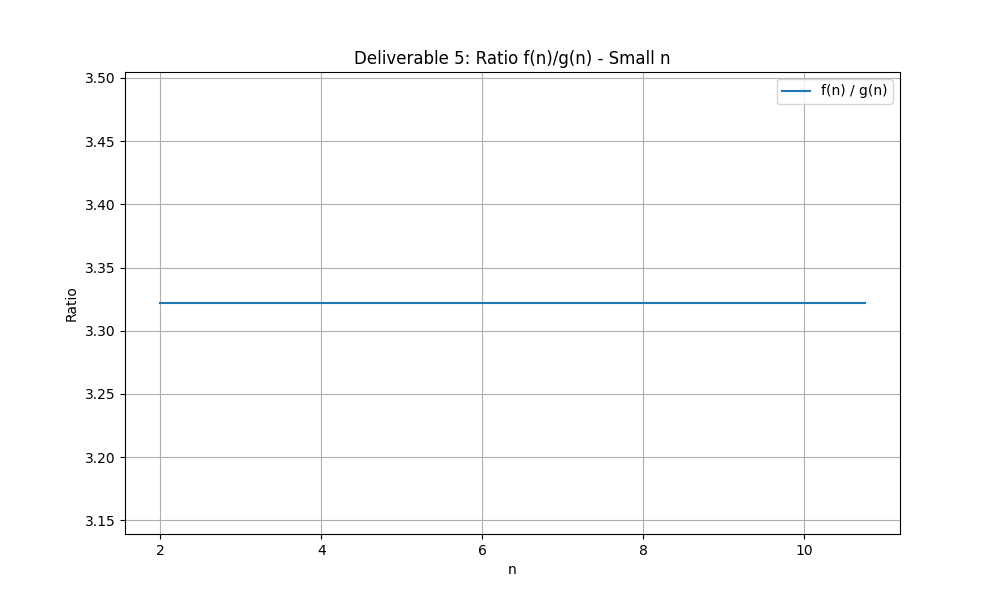
\includegraphics[width=\textwidth]{plot_deliverable5_ratio_smalln.png}
    \caption{Plot of $\frac{f(n)}{g(n)}$ for $n$ ranging from 2 to 10.}
    \label{fig:ratio_fn4_gn4_2_10}
\end{figure}

\begin{figure}[H]
    \centering
    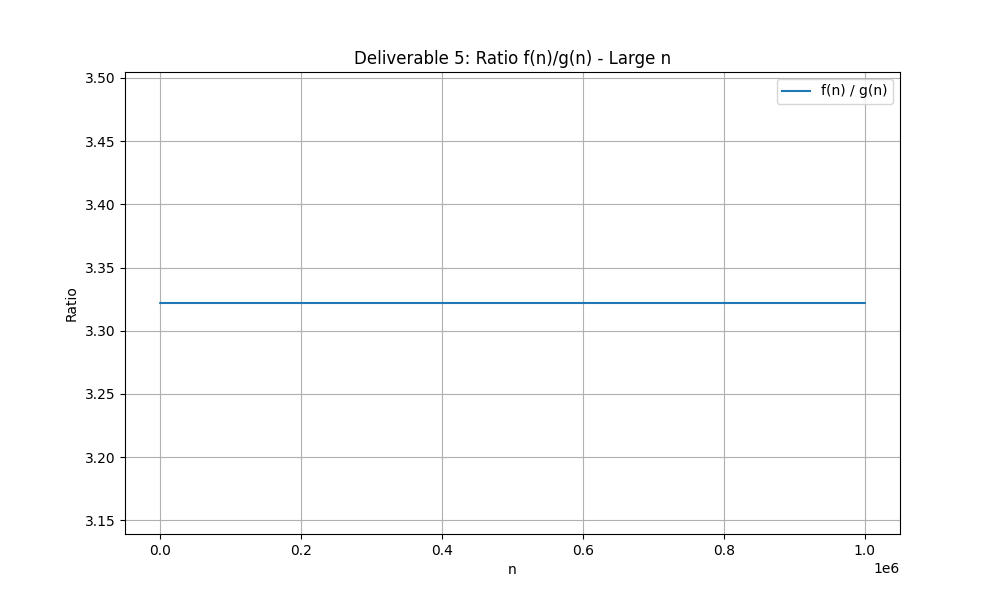
\includegraphics[width=\textwidth]{plot_deliverable5_ratio_largen.png}
    \caption{Plot of $\frac{f(n)}{g(n)}$ for $n$ ranging from 2 to $10^6$.}
    \label{fig:ratio_fn4_gn4_2_10e6}
\end{figure}

\textbf{Interpretation:} As expected, both $f(n)$ and $g(n)$ grow at the same rate. The ratio plots confirm that the ratio is a constant for both small and large $n$, indicating that both functions are in the same order of growth, $\Theta(\log n)$. Interestingly, at first it looked like $\log_2 n$ grew faster. However, I believe this was because $\log_2 n$ needs more digits to represent the same numbers, so it settles around a higher number on the y-axis.

\section{Conclusion}

This project successfully demonstrates how different functions can be analyzed and compared in terms of their asymptotic growth rates. By plotting the functions and their ratios over various ranges, we were able to visually become more comfortable with the different orders of growth.

\end{document}